\documentclass[10pt]{article}
\usepackage[utf8]{inputenc}

\usepackage{latexsym}
\usepackage{amssymb,amsmath}
\usepackage{graphicx}
\usepackage{sgame}
\usepackage{color}
\usepackage{authblk}

\usepackage[hidelinks]{hyperref}
\usepackage{empheq}
\usepackage{blkarray}
\usepackage{cancel}
\usepackage{enumerate}
\usepackage{times}
\usepackage{array}
\usepackage{lscape}
\usepackage{xcolor}

\usepackage[margin=1in]{geometry}
\newcommand{\newword}[1]{\textbf{\emph{#1}}}

%Arrows
\newcommand{\into}{\hookrightarrow}
\newcommand{\onto}{\twoheadrightarrow}

%Things LaTeX names by appearance, rather than meaning
\newcommand{\isom}{\cong} %The isomorphism symbol
\newcommand{\union}{\cup}
\newcommand{\intersection}{\cap}
\newcommand{\bigunion}{\bigcup}
\newcommand{\bigintersection}{\bigcap}
\newcommand{\disjointunion}{\sqcup}
\newcommand{\bigdisjointunion}{\bigsqcup}

\newcommand\numberthis{\addtocounter{equation}{1}\tag{\theequation}}

%Some multiletter functions
\DeclareMathOperator{\Hom}{Hom}
\DeclareMathOperator{\Ext}{Ext}
\DeclareMathOperator{\End}{End}
\DeclareMathOperator{\Tor}{Tor}
\DeclareMathOperator{\Ker}{Ker}
\DeclareMathOperator{\CoKer}{CoKer}
\DeclareMathOperator{\Spec}{Spec}
\DeclareMathOperator{\Proj}{Proj}
\renewcommand{\Im}{\mathop{\mathrm{Im}}}
%Their calligraphic versions; use these for the sheaf constructions
\DeclareMathOperator{\HHom}{\mathcal{H} \textbf{om}}
\DeclareMathOperator{\EExt}{\mathcal{E} \textbf{xt}}
\DeclareMathOperator{\EEnd}{\mathcal{E} \textbf{nd}}
\DeclareMathOperator{\TTor}{\mathcal{T} \textbf{or}}
\DeclareMathOperator{\KKer}{\mathcal{K}\textbf{er}}
\DeclareMathOperator{\CCoKer}{\mathcal{C} \textbf{o}\mathcal{K} \textbf{er}}
\newcommand{\IIm}{\mathop{\mathcal{I} \textbf{m}}}
\newcommand{\ccH}{\mathscr{H}} %The very curly H

\DeclareMathOperator{\sss}{\mathrm{sunny}}
\DeclareMathOperator{\rrr}{\mathrm{rainy}}
\DeclareMathOperator{\hhh}{\mathrm{hot}}
\DeclareMathOperator{\ccc}{\mathrm{cold}}

%This makes alternating tensors look right in displayed equations
\newcommand{\Alt}{\bigwedge\nolimits}

%Blackboard bold letters
\renewcommand{\AA}{\mathbb{A}}
\newcommand{\BB}{\mathbb{B}}
\newcommand{\CC}{\mathbb{C}}
\newcommand{\DD}{\mathbb{D}}
\newcommand{\EE}{\mathbb{E}}
\newcommand{\FF}{\mathbb{F}}
\newcommand{\GG}{\mathbb{G}}
\newcommand{\HH}{\mathbb{H}}
\newcommand{\II}{\mathbb{I}}
\newcommand{\JJ}{\mathbb{J}}
\newcommand{\KK}{\mathbb{K}}
\newcommand{\LL}{\mathbb{L}}
\newcommand{\MM}{\mathbb{M}}
\newcommand{\NN}{\mathbb{N}}
\newcommand{\OO}{\mathbb{O}}
\newcommand{\PP}{\mathbb{P}}
\newcommand{\QQ}{\mathbb{Q}}
\newcommand{\RR}{\mathbb{R}}
\renewcommand{\SS}{\mathbb{S}}
\newcommand{\TT}{\mathbb{T}}
\newcommand{\UU}{\mathbb{U}}
\newcommand{\VV}{\mathbb{V}}
\newcommand{\WW}{\mathbb{W}}
\newcommand{\XX}{\mathbb{X}}
\newcommand{\YY}{\mathbb{Y}}
\newcommand{\ZZ}{\mathbb{Z}}

%Calligraphic letters

\newcommand{\cA}{\mathcal{A}}
\newcommand{\cB}{\mathcal{B}}
\newcommand{\cC}{\mathcal{C}}
\newcommand{\cD}{\mathcal{D}}
\newcommand{\cE}{\mathcal{E}}
\newcommand{\cF}{\mathcal{F}}
\newcommand{\cG}{\mathcal{G}}
\newcommand{\cH}{\mathcal{H}}
\newcommand{\cI}{\mathcal{I}}
\newcommand{\cJ}{\mathcal{J}}
\newcommand{\cK}{\mathcal{K}}
\newcommand{\cL}{\mathcal{L}}
\newcommand{\cM}{\mathcal{M}}
\newcommand{\cN}{\mathcal{N}}
\newcommand{\cO}{\mathcal{O}}
\newcommand{\cP}{\mathcal{P}}
\newcommand{\cQ}{\mathcal{Q}}
\newcommand{\cR}{\mathcal{R}}
\newcommand{\cS}{\mathcal{S}}
\newcommand{\cT}{\mathcal{T}}
\newcommand{\cU}{\mathcal{U}}
\newcommand{\cV}{\mathcal{V}}
\newcommand{\cW}{\mathcal{W}}
\newcommand{\cX}{\mathcal{X}}
\newcommand{\cY}{\mathcal{Y}}
\newcommand{\cZ}{\mathcal{Z}}


\DeclareMathOperator{\ord}{ord}
\DeclareMathOperator{\inte}{int}
\DeclareMathOperator{\nhd}{nhd}

\newcommand{\ds}{\displaystyle}
\newcommand{\mc}{\mathcal}
\newcommand{\ol}{\overline}
\newcommand{\modu}{\hspace{-2mm} \mod}

\DeclareMathOperator{\inn}{Inn}
\DeclareMathOperator{\aut}{Aut}
\DeclareMathOperator{\cen}{Center}
\DeclareMathOperator{\im}{Im}
\DeclareMathOperator{\re}{Re}
\DeclareMathOperator{\id}{id}
\DeclareMathOperator{\mor}{Mor}
\DeclareMathOperator{\irr}{Irr}
\DeclareMathOperator{\sgn}{sgn}

\DeclareMathOperator{\cov}{Cov}
\DeclareMathOperator{\var}{Var}

\DeclareMathOperator{\erf}{erf}
%\DeclareMathOperator{\sgn}{sgn}
\DeclareMathOperator{\argmin}{argmin}
\DeclareMathOperator{\argmax}{argmax}

\DeclareMathOperator{\lip}{Lip}

\newcommand{\bbm}{\begin{bmatrix}}
\newcommand{\bpm}{\begin{pmatrix}}
\newcommand{\ebm}{\end{bmatrix}}
\newcommand{\epm}{\end{pmatrix}}

\newcommand{\ddx}[2]{\frac{d #1}{d #2}}
\newcommand{\ddt}[1]{\frac{d #1}{dt}}

 \newcommand{\del}[2]{\frac{\partial #1}{\partial #2}}
 \newcommand{\dsdel}[2]{\displaystyle\frac{\partial #1}{\partial #2}}
 
 \newcommand{\doubledel}[3]{\displaystyle\frac{\partial^2 #1}{\partial #2 \partial #3}}
 \newcommand{\doubledelsame}[2]{\displaystyle\frac{\partial^2 #1}{\partial #2^2}}
  
%newcommand{\ddx}[2]{\frac{d #1}{d #2}}
%\newcommand{\ddt}[1]{\frac{d #1}{dt}}

\newcommand{\dsddx}[2]{\displaystyle\frac{d #1}{d #2}}
\newcommand{\dsddt}[1]{\displaystyle\frac{d #1}{dt}}

\newcommand{\pbderiv}{\ds\del{V}{x_1} \dsddt{x_1} + \ds\del{V}{x_2} \dsddt{x_2}}

\newcommand{\ito}{It\^o \hspace{0.05mm}}
\newcommand{\itos}{It\^os \hspace{0.05mm}}

\newcommand{\gronwall}{Gr\"onwall  \hspace{0.05mm}}
\newcommand{\gronwalls}{Gr\"onwall's  \hspace{0.05mm}}

\newcommand{\tw}{d\tilde{W}_t}
\newcommand{\tws}{d\tilde{W}_s}

\newcommand{\A}{{\color{red}A}}
\newcommand{\B}{{\color{blue}B}}

\bibliographystyle{plain}
\usepackage{float}


%%%%%%%%%%%%%%%%%%%%%%%%%%%
% Document-specific settings

\title{\vspace{-30pt}\Large Analytical Mixing Model, v2\vspace{-10pt}}
\author{Mari Kawakatsu\vspace{-15pt}}
\date{Last updated: \today\vspace{-15pt}}

\graphicspath{ {../output/Task_dist/} }
\usepackage[margin=.3in]{caption}

%%%%%%%%%%%%%%%%%%%%%%%%%%%
\begin{document}

\maketitle

\tableofcontents

\section{Overview}
\begin{itemize}
    \item Following up on the last Skype with Yuko \& Daniel, I ran additional simulations in which I varied a combination of parameters, namely the task efficiencies $\alpha$ and the demand rates $\delta$ (results on slides).
    
    \item There seemed to be some strange behavior when at least one of the lines was inefficient. To understand what was happening, I decided to write down equations that approximate the computational model to gain insight into the (expected) steady-state behavior (see Sections~\ref{sec:model} and \ref{sec:ss}).
    
    \item A preliminary analysis of the model seems to suggest that, assuming that the system reaches/has a steady state, varying only $\delta$ and $\alpha$ can result in a downward contagion but not an upward contagion (see Section~\ref{sec:contagion}). If this is true, then in order for the FTM to capture the experimental data, it must be the case that the two genetic lines differ in some trait other than their task efficiency.
    
    \item (Update 2/9) I extended the model to capture non-50-50 mixes (highlighted in {\color{orange}orange}).
    
\end{itemize}

\section{Model} \label{sec:model}

To consider the dynamics of division of labor in mixed colonies, we extend the fixed threshold model in \cite{ulrich18} to incorporate ants of two genetic lines, \A\ and \B. 

The model considers $n$ individuals and $m$ tasks. 
{\color{orange}Let $f$ and $1=f$ be the fractions of genetic line \A\ and \B\ individuals in the colony, respectively.}
% The $n$ individuals consist of equal numbers of genetic line \A\ and genetic line \B\ individuals.
We assume that each task $j$ has an associated stimulus, $s_{j,t}$, at every time $t$, indicating group-level demand for that task. We model the change in stimulus over discrete time as
\begin{equation}
    s_{j,t+1} - s_{j,t} = \delta_j - \frac{\alpha_j^{\A} x_{j,t}^{\A} + \alpha_j^{\B} x_{j,t}^{\B} }{n}, \label{eq:stim}
\end{equation}
where 
\begin{itemize}
    \item $\delta_j$ is the task-specific demand rate;
    \item $\alpha_j^{\A}$ and $\alpha_j^{\B}$ are the task-specific performance efficiencies of lines \A\ and \B, respectively; and
    \item $x_{j,t}^{\A}$ and $x_{j,t}^{\B}$ are the numbers of line \A\ and line \B\ individuals performing task $j$ and time $t$, respectively.
\end{itemize}

At each time step, inactive individuals are exposed to the task stimuli randomly until either they begin performing a task or they have encountered all stimuli without landing on a task. Similar to \cite{ulrich18}, our computational model draws individual $i$'s internal threshold for task $j$, $\theta_{ij}$, from a normal distribution with mean $\mu_j$ and normalized standard deviation $\sigma_j$ (each of these parameters can be line- and/or task-specific). \textit{To gain analytical insight into the model, we make the simplifying assumption that the line- and task-specific thresholds are given by the constant parameters, $\mu_j^{\A}$ and $\mu_j^{\B}$.}

With this assumption, the probabilities $P_{ij,t}^{\A}$ and $P_{ij,t}^{\B}$ that individuals $i$ of lines \A\ and \B, respectively, perform task $j$ at time $t$ can be written as
\begin{equation}
    P_{j,t}^{\A} (s_{j,t}) = \frac{s_{j,t}^\eta}{s_{j,t}^\eta + {(\mu_j^{\A})}^\eta}, \quad P_{j,t}^{\B} (s_{j,t}) = \frac{s_{j,t}^\eta}{s_{j,t}^\eta +{(\mu_j^{\B})}^\eta},
\end{equation}
where $\eta$ is the threshold response parameter as in the original model. Finally, at a given time $t$, active individuals quit their tasks with a constant quit probability $\tau$. In the case of two tasks ($m = 2$), the change in the number of line \A\ and line \B\ individuals working on task $j$ is given by\footnote{explain this more in English}
\begin{align}
    x_{j,t+1}^{\A} - x_{j,t}^{\A} & = \frac{1}{2} \bigg[ P_{j,t}^{\A}(s_{j,t}) + (1 - P_{j',t}^{\A}(s_{j',t}))P_{j,t}^{\A}(s_{j,t})\bigg] \bigg( {\color{orange}fn}
 - (x_{j,t}^{\A} + x_{j',t}^{\A}) \bigg) - \tau x_{j,t}^{\A} \nonumber\\
    x_{j,t+1}^{\B} - x_{j,t}^{\B} & = \frac{1}{2} \bigg[ P_{j,t}^{\B}(s_{j,t}) + (1 - P_{j',t}^{\B}(s_{j',t}))P_{j,t}^{\B}(s_{j,t})\bigg] \bigg( {\color{orange}(1-f)n} - (x_{j,t}^{\B} + x_{j',t}^{\B}) \bigg) - \tau x_{j,t}^{\B} \label{eq:active}
\end{align}
for $(j,j')=(1,2), (2,1)$. {\color{orange}The sums in square brackets capture the possible ways in which individuals can initiate task $j$: they can either encounter the stimulus for task $j$ immediately and begin performing that task, or they can first encounter the stimulus for the other task $j'$, decide not to perform that task, subsequently encounter the stimulus for task $j$, and begin performing task $j$.}

The full model for $m=2$ consists of the six equations describing changes in $s_1, s_2$ (Eq.~\eqref{eq:stim}) and $ x_1^{\A}, x_1^{\B}, x_2^{\A}, x_2^{\B}$ (Eq.~\eqref{eq:active}), {\color{orange}under the constraints $x_{1,t}^{\A}+x_{2,t}^{\A} \leq fn$ and $x_{1,t}^{\B}+ x_{2,t}^{\B} \leq (1-f)n$}.

\section{Steady-state predictions} \label{sec:ss}
One way to understand what is happening in the simulations is to consider the equilbria of the above model. My intent here is not (yet) to prove the stability etc. rigorously but to get a sense for what we should expect to see in the simulations.

\subsection{Pure colonies: 2 tasks, 1 line}
For pure (\A-only) colonies, we set $x_{j,t}^{\B} = 0$ for all time $t$. Setting Eq.~\eqref{eq:stim} to zero, we obtain
\begin{equation}
    \frac{x_j^{\A}}{n} = \frac{\delta_j}{\alpha_j^{\A}}
    \label{eq:ss1}
\end{equation}
as the fraction of (\A) ants that are performing task $j$ ($j = 1,2$) at steady state. We can us this to compute the steady-state levels of stimuli if needed.

\textbf{Notably, the steady-state values of $x_j^{\A}$ are \textbf{independent} of the mean threshold ($\mu_j^{\A}$) or the quit probability ($\tau^{\A}$). This agrees with the results of our simulations, where varying $\mu$ and $\tau$ by line did not lead to differing mean task performance levels in the pure colonies.}

Note that the sum of the fractions \eqref{eq:ss1} across tasks should not exceed one. So a necessary condition for the steady-state to be biologically realizable is 
\begin{equation}
    \frac{x_1^{\A}}{n} + \frac{x_2^{\A}}{n} = \frac{\delta_1}{\alpha_1^{\A}} + \frac{\delta_2}{\alpha_2^{\A} }\leq 1 \label{eq:cond1}.
\end{equation}
If this condition is not met, then we would expect the stimuli to continue growing (i.e., the system will not reach a steady state). \textbf{A ``symptom'' of this phenomenon, I think, is that the ants become ``maxed out'' (I can explain this more when we Skype)}.

\subsection{Mixed colonies: 2 tasks, 2 lines, 50-50 mixes}

{\color{orange}We first consider the 50-50 mixes ($f=0.5$), i.e. mixed colonies consisting of an equal number of \A\ and \B\ ants.}
Moreover, we assume that the mean thresholds and the quit probabilities are identical for both tasks and lines ($\mu_1^{\A} = \mu_2^{\A} = \mu_1^{\B} = \mu_2^{\B}$ and $\tau^{\A} = \tau^{\B}$), as we have done in the simulations with varied $\delta$ and $\alpha$ values. Setting Eq.~\eqref{eq:stim} and Eq.~\eqref{eq:active} equal to zero, we find\footnote{This is the expression I get when I set $1\leq \eta \leq 20, \eta \in \ZZ$. There seems to be something numerically tricky when $\eta$ takes non-integer values.} the expression for the steady-state numbers of individuals performing task $j$:%\footnote{}
\begin{equation}
     x_j^{\A} =  x_j^{\B} = n\bigg(\frac{\delta_j}{\alpha_j^{\A} + \alpha_j^{\B}}\bigg) \label{eq:ss2a}
\end{equation}
for $j = 1, 2$.
Alternatively, as fractions of each genetic type of individuals,
\begin{equation}
     \frac{x_j^{\A}}{(n/2)} =  \frac{x_j^{\B}}{(n/2)} = \frac{2\delta_j}{\alpha_j^{\A} + \alpha_j^{\B}}. \label{eq:ss2}
\end{equation}
The necessary condition for this steady state to exist is
\begin{equation}
     \sum_{j=1}^2 \frac{x_j^{\A}}{n} + \frac{x_j^{\B}}{n} 
     = \sum_{j=1}^2 \frac{2\delta_j}{\alpha_j^{\A} + \alpha_j^{\B}}
     \leq 1.
     \label{eq:cond2}
\end{equation}
Again, if this condition is not met, then we would expect the stimuli to continue growing over time and for the ants to be working at max capacity.

While $\mu$ doesn't explicitly appear in the expression \eqref{eq:ss2} when we assume that the mean thresholds are identical for all individuals and both tasks, we expect\footnote{I haven't been able to get Mathematica to compute the expressions explicitly, but we can infer this from the form of the threshold functions.} the general form of steady state fractions of active individuals to be functions of $\mu_j^{\A}$ and $\mu_j^{\B}$ as well as $\tau^{\A}$ and $\tau^{\B}$. \textbf{So one question to investigate using simulations (numerical or computational) would be \textbf{how the mean thresholds ($\mu$) interact with either the demand rates ($\delta$) or the task efficiencies ($\alpha$)}.}

\subsubsection{Comparing with simulation results}

{\color{orange}
\subsection{Mixed colonies: 2 tasks, 2 lines, non-50-50 mixes (NEW)}
We now generalize to the case in which a fraction $f$ of individuals in a mixed colony are of genetic line} \A. In the simplified case where $\mu_1^{\A} = \mu_2^{\A} = \mu_1^{\B} = \mu_2^{\B}$ and $\tau^{\A} = \tau^{\B}$, the steady-state fractions of individuals performing task $j$ are
\begin{equation}
     x_j^{\A} =  \frac{fn\delta_j}{f\alpha_j^{\A} + (1-f)\alpha_j^{\B}}, 
     \quad
     x_j^{\B} =  \frac{(1-f)n\delta_j}{f\alpha_j^{\A} + (1-f)\alpha_j^{\B}}, 
     \label{eq:ss3a}
\end{equation}
or, as fractions of the individuals of each genetic type (recall that there are $fn$ individuals of type \A\ and $(1-f)n$ individuals of type \B),
\begin{equation}
     \frac{x_j^{\A}}{fn} =  \frac{x_j^{\B}}{(1-f)n} = \frac{\delta_j}{f\alpha_j^{\A} + (1-f)\alpha_j^{\B}} \ \bigg(= \frac{x_j^{\A} + x_j^{\B}}{n}\bigg). \label{eq:ss3}
\end{equation}
The last equality highlights the fact that the fraction of individuals \textit{of each type} performing task $j$ is identical to the fraction \textit{of the whole colony} performing that task. As expected, the expressions \eqref{eq:ss3} reduce to \eqref{eq:ss2} when $f=0.5$ (50-50 mixes) and to \eqref{eq:ss1} when $f=1$ (pure \A\ colonies).

Again, we would expect to see this equilibria only when $x_1^{\A} + x_1^{\B} + x_2^{\A}+ x_2^{\B} \leq n$ is satisfied.

{\color{orange}
From these results, we would expect the steady-state fraction of task $j$ performance frequency (which corresponds to \eqref{eq:ss3}) to depend \textbf{nonlinearly} on the fraction of \A\ individuals ($f$). 
}

\subsubsection{Comparing with simulation results}
\begin{figure}[H]
    \centering
    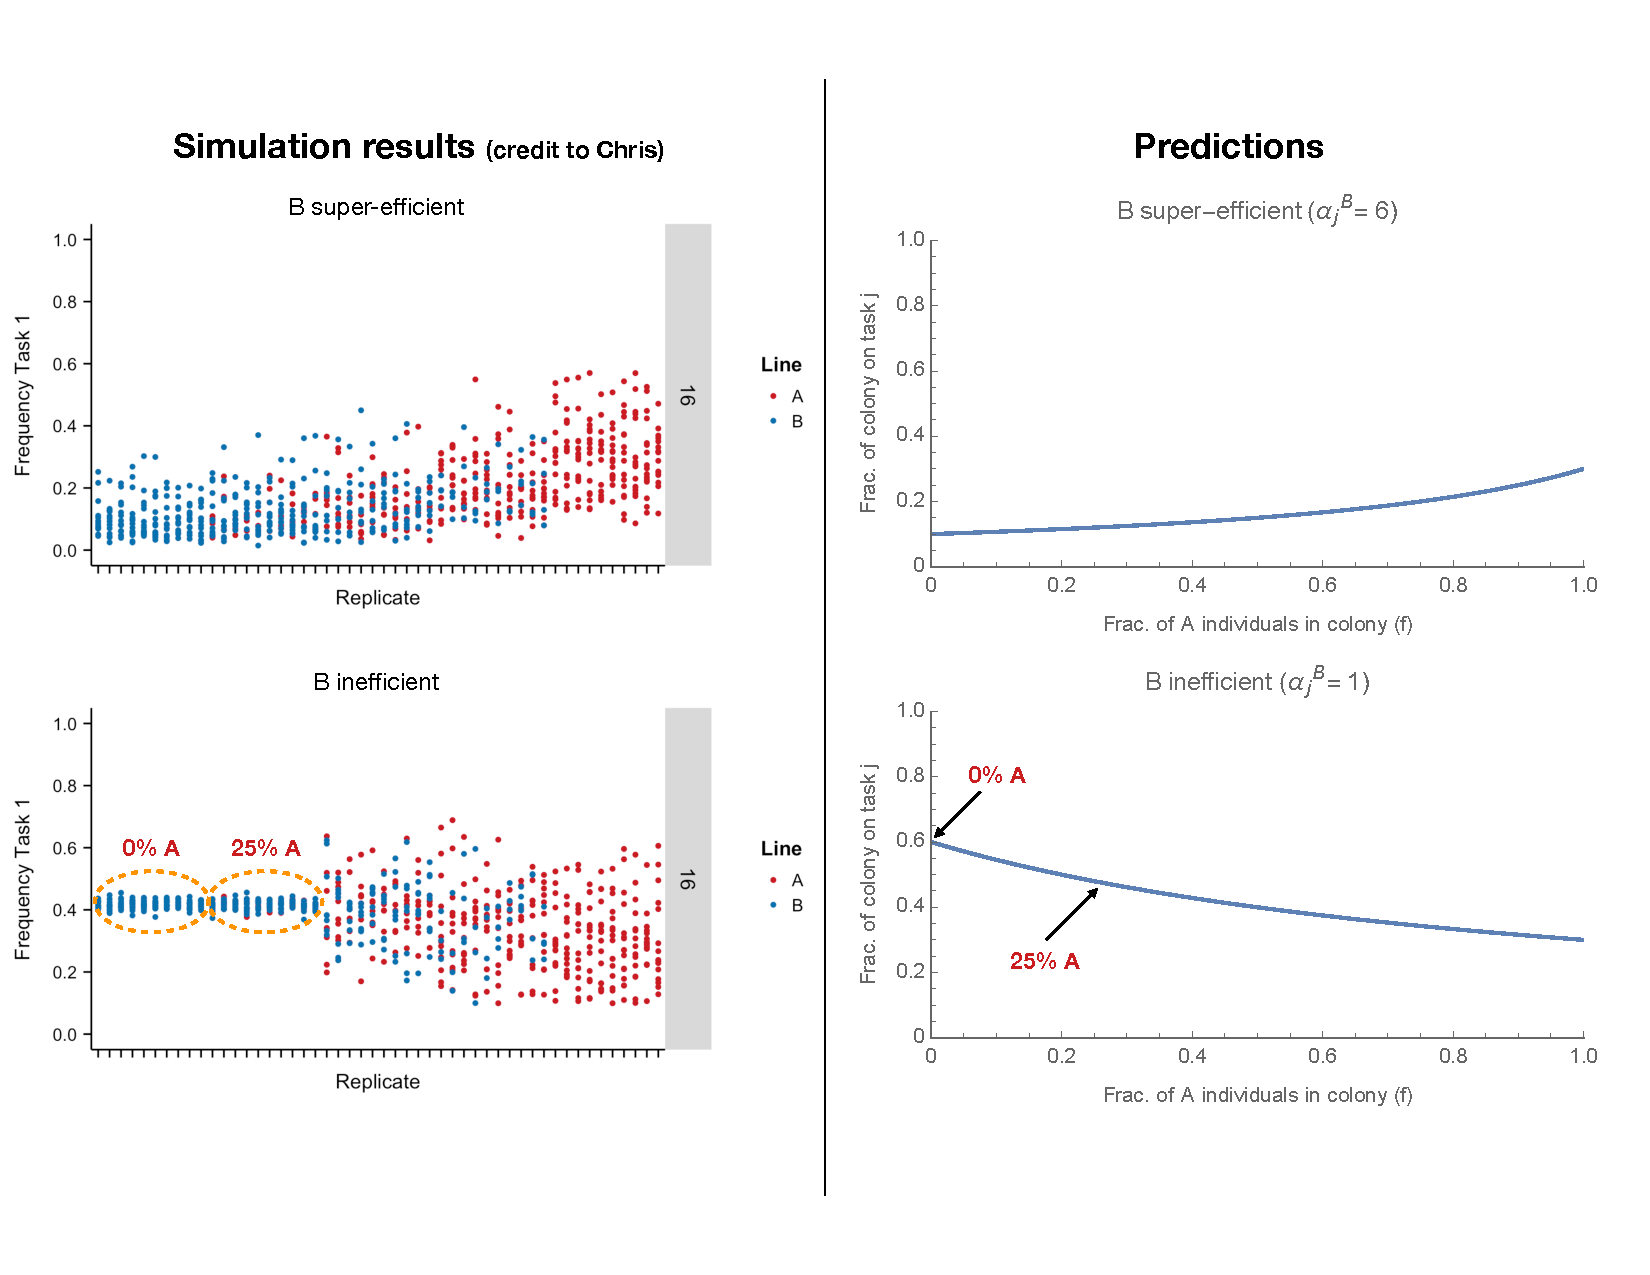
\includegraphics[trim={0 1in 0 0.75in}, clip, width=0.95\linewidth]{output/Task_dist/mixes_comparison.pdf}
    \caption{Comparison of simulation results (left) and analytical predictions of steady states (right) according to the model above. The parameters used in both columns are as follows: $\alpha_1^{\A} = \alpha_2^{\A} = 2, \delta= 0.6, \mu=10, \sigma = 0.1$. 
    \textbf{Top row}: The \B\ ants are ``super-efficient'' at both tasks ($\alpha_1^{\B} = \alpha_2^{\B} = 2$, top row). In the simulations, task performance \textit{increases nonlinearly} as the fraction of \A\ ants in the colony increases (left), as predicted qualitatively by the model (right).
    \textbf{Bottom row}: The \B\ ants are ``inefficient'' at both tasks ($\alpha_1^{\B} = \alpha_2^{\B} = 1$). 
    Similar to the 50-50 cases, when the colony primarily consists of the inefficient \B\ ants ($f = 0, 0.25$ in the simulations), the model \textit{overpredicts} the colony activity.
    Where there are sufficiently many \A\ ants in the colony ($f = 0.5, 0.75, 1$ in the simulations), however, both the simulations and model predictions show a \textit{nonlinear negative} relationship in task performance.}
    \label{fig:mixes_comp}
\end{figure}

\section{Downward vs. upward contagion in the 50-50 mixes} \label{sec:contagion}

A focus during our last Skype with Daniel and Yuko was how the model could qualitatively capture the two contagion patterns in Fig.~1 (bottom row) of Yuko's document. Specifically, they were interested in \textbf{whether varying both the task efficiencies $\alpha$ and the demand rates $\delta$ would capture the difference in the directions of contagion (downward or upward) when the larvae differed.}

Here's my conclusion so far: {\color{red}\textit{If we assume that the system reaches its steady state within the observed period (i.e., conditions \eqref{eq:cond1} and \eqref{eq:cond2} are satisfied\footnote{This part is technically not tight, since I haven't analyzed what the sufficient conditions are}), then varying \textbf{only} $\delta$ and $\alpha$ can result in a downward contagion but not an upward contagion.}}

Here's why I think this is the case: If we only vary $\delta$ and $\alpha$, then the mean thresholds and the quit probabilities are identical across tasks and lines. So we can directly apply the steady-state fractions of active individuals computed in Eqs.~\eqref{eq:ss1} and \eqref{eq:ss2}. In this case, the behavioral contagion is ``downward'' if
\begin{equation}
    \frac{1}{2} \bigg( \frac{\delta_j}{\alpha_j^{\A}} + \frac{\delta_j}{\alpha_j^{\B}} \bigg) > \frac{2\delta_j}{\alpha_j^{\A} + \alpha_j^{\B}} \label{eq:down}
\end{equation}
and ``upward'' if the inequality is reversed (the schematic below should help).
\begin{figure}[H]
    \centering
    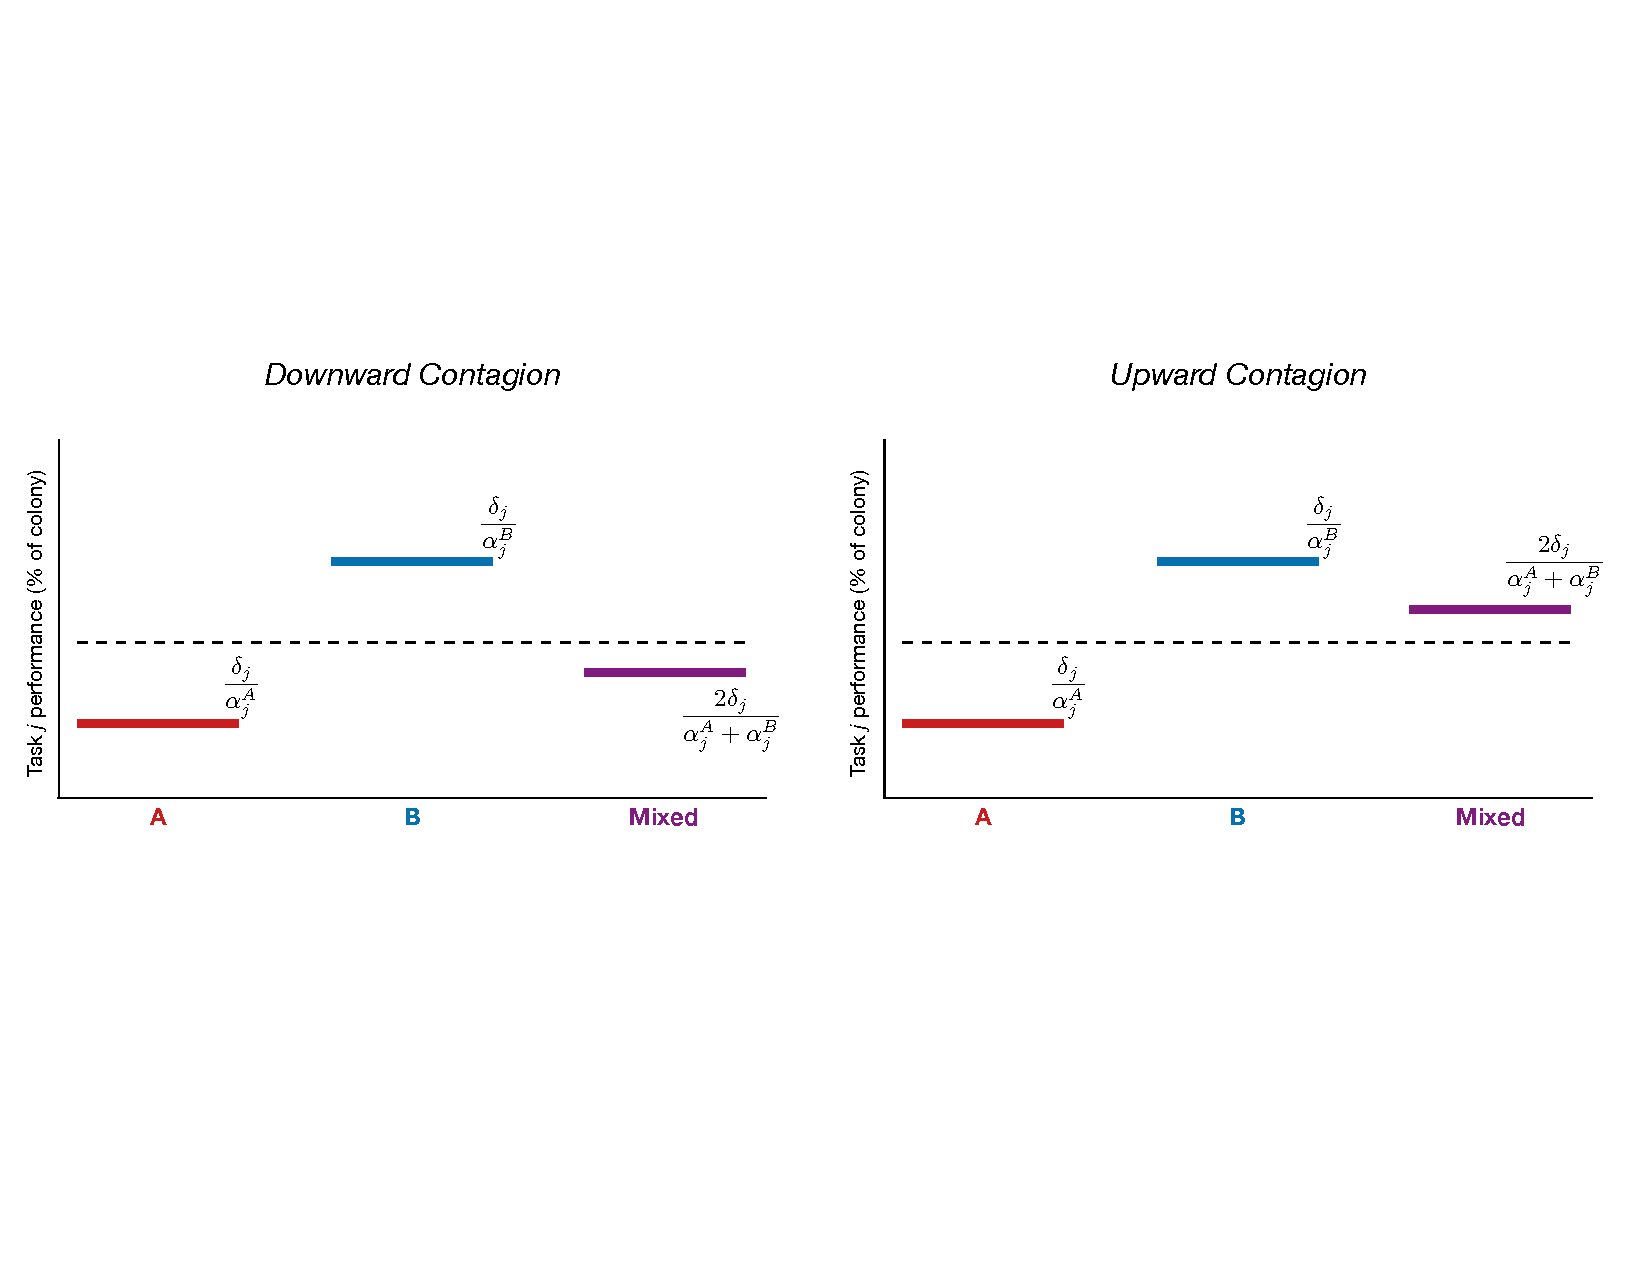
\includegraphics[width=0.9\linewidth]{doc/schematic_contagion.pdf}
    \caption{A schematic representing the two contagion patterns of our interest. The task $j$ performance (\%) values for the mixed colonies assume that the mean thresholds and the quit probabilities are identical for both lines and both tasks ($\mu_1^{\A} = \mu_2^{\A} = \mu_1^{\B} = \mu_2^{\B}$) and ($\tau^{\A} = \tau^{\B}$).}
    \label{fig:schematic}
\end{figure}
By manipulating the inequality \eqref{eq:down}, however, we see that \textbf{only the downward contagion is possible} under our assumptions:
\begin{align}
    \frac{1}{2} \bigg( \frac{\delta_j}{\alpha_j^{\A}} + \frac{\delta_j}{\alpha_j^{\B}} \bigg) - \frac{2\delta_j}{\alpha_j^{\A} + \alpha_j^{\B}} 
    & = \frac{\delta_j}{2} \bigg( \frac{1}{\alpha_j^{\A}} + \frac{1}{\alpha_j^{\B}} - \frac{4}{\alpha_j^{\A} + \alpha_j^{\B}} \bigg) \nonumber\\
    & = \frac{\delta_j}{2} \Bigg( 
    \frac{\alpha_j^{\B} (\alpha_j^{\A} + \alpha_j^{\B}) + \alpha_j^{\A} (\alpha_j^{\A} + \alpha_j^{\B}) - 4\alpha_j^{\A}\alpha_j^{\B}}{\alpha_j^{\A}\alpha_j^{\B}(\alpha_j^{\A} + \alpha_j^{\B})} \Bigg) \nonumber\\
    & = \frac{\delta_j}{2} \Bigg( 
    \frac{ (\alpha_j^{\A})^2 + (\alpha_j^{\B})^2 - 2\alpha_j^{\A}\alpha_j^{\B}}{\alpha_j^{\A}\alpha_j^{\B}(\alpha_j^{\A} + \alpha_j^{\B})} \Bigg) 
    = \frac{\delta_j}{2} \Bigg( 
    \frac{ (\alpha_j^{\A} - \alpha_j^{\B})^2 }{\alpha_j^{\A}\alpha_j^{\B}(\alpha_j^{\A} + \alpha_j^{\B})} \Bigg) > 0
\end{align}

Upward contagion is still possible if we relax some of our assumptions. In the simulations I've run so far, upward contagion appears
\begin{itemize}
    \item when the mean thresholds ($\mu$) are varied in addition to the task efficiencies ($\alpha$), or
    \item when at least one of the lines is not sufficiently efficient to maintain the stimuli at constant levels (i.e., reach steady state).
\end{itemize}

\section{Questions}
\begin{itemize}
    \item How reasonable is it to assume that the empirically observed behavior corresponds to the steady state of the model? {\color{orange}Need to make this assumption for steady-state analysis, but should also consider cases where this assumption does not hold and }
    
    \item From our earlier simulations, we know that both the mean threshold ($\mu$) or the quit probability ($\tau$) lead to ``behavioral amplification'' in the mixed case.
    Biologically speaking, which is more likely to vary by genetic line? Also, what happens when $\alpha$ AND either $\mu$ and $\tau$ are varied?
    
    \item What do these ``upward'' and ``downward'' contagions imply? As in, why might they be biologically interesting? {\color{orange}We will ask Yuko et al. when we send them the summary document.}
\end{itemize}

\begin{thebibliography}{99}

\bibitem{ulrich18} Y. Ulrich, J. Saragosti, C. K. Tokita, C. E. Tarnita, D. J. C. Kronauer, ``Fitness benefits and emergent division of labour at the onset of group living,'' \textit{Nature}, vol. 560, pp. 635-638, Aug. 2018.

\end{thebibliography}

\end{document}
%%%%%%%%%%%%%%%%%%%%%%%%%%%

